\begin{frame}
\frametitle{Basic Regression}

\begin{equation}
\label{equ:ExLinEqu}
y = a_0 + a_1 x
\end{equation}

\begin{equation}
\label{equ:LSE_E2}
E^2 = \sum_{i=1}^{n} (y_i - y)^2
\end{equation}

\begin{equation}
\label{equ:LSE_E2b}
E^2 = \sum_{i=1}^{n} (y_i - (a_0 + a_1 x_i))^2
\end{equation}

\begin{align} 
    \frac{\partial E^2}{\partial a_0} &= 0 = \sum_{i=1}^{n} (-2y_i +2a_0 + 2a_1 x_i)           \label{equ:LSE_PD1} \\
    \frac{\partial E^2}{\partial a_1} &= 0 = \sum_{i=1}^{n} (-2y_i x_i +2a_0 x_i + 2a_1 x_i^2) \label{equ:LSE_PD2}
\end{align}

\end{frame}

\begin{frame}
\begin{figure}[ht!]
\ifisPPT
\noindent\makebox[\textwidth]{\includegraphics[keepaspectratio=true,width=\paperwidth]{../figures/regression/basicLSE.jpg}}
\else
\includegraphics[keepaspectratio=true,width=6in]{./figures/regression/basicLSE.jpg}
\fi
\centering
\caption{Basic LSE}
\label{fig:basicLSE}
\end{figure}


\end{frame}

